\def\Ponderation{35}
\def\SigleNumero{STT-1000}
\def\NomCours{Probabilités et statstique}
\def\DateEvaluation{16 décembre 2024}
\def\HeureEvaluation{18h30 à 21h20}
\def\Session{}
\def\NomEvaluation{Examen 2}

% Ne rien mettre entre les accolades si l'enseignant (ou l'enseignante) est aussi le coordonnateur (ou la coordonnatrice)
\def\Coordonnatrice{}
\def\Coordonnateur{}

% Ne rien mettre entre les accolades s'il y a plus d'une section
\def\Enseignant{}
\def\Enseignante{}

% Ne rien mettre entre les accolades s'il s'agit d'un cours à section unique
% Mettre le nom de chacun des enseignants et enseignantes entre les accolades
% Une case à cocher sera générée pour chacune des sections
\def\SectionA{Rachid Kandri-Rody}
\def\SectionB{Julien Miron}
\def\SectionC{}
\def\SectionD{}


\def\Directives{
\begin{enumerate}
\item Matériel autorisé:
\begin{itemize}
\item Calculatrice scientifique {\bf autorisée par la faculté des sciences et de génie};
\item Le feuillet de formules fourni avec l'examen. Celui-ci inclut les tables dont vous aurez besoin. Veuillez ne rien écrire sur le feuillet de formules.
\end{itemize}
\item Assurez-vous que cette évaluation comporte \numquestions ~exercices répartis sur \numpages{}~pages, pour un total de \numpoints{}~points.\
\item \textbf{Veuillez ne pas dégrafer votre examen.}
\item Ajoutez vos initiales dans le bas de chaque page.
\item Vous devez\textbf{ justifier toutes vos réponses} par une démarche claire, sauf pour les questions à choix de réponse.\
\item Lorsque des boîtes de réponses sont présentes, vous \textbf{\textit{devez}} y écrire vos réponses. N'écrivez que la réponse (aucun nom de variable ou unité de mesure).\
\item Pour les questions à choix de réponse et les vrais ou faux, vous pouvez mettre un X, un crochet ($\checkmark$) ou remplir la case.\
\item Certains vrais ou faux demande une justification. Aucun point ne sera donné sans justification, même si vous cochez la bonne réponse.
\item Pour les questions à choix de réponse, lorsqu'il est écrit «cochez tous les énoncés qui sont vrais/faux», il est possible qu'un seul énoncé soit vrai.
\item Le verso des feuilles peut être utilisé comme brouillon, \textbf{mais ne sera pas corrigé}. Attention à ne rien dégrafer.
\end{enumerate}
}



\documentclass{Evaluation}
\usepackage{multicol,graphicx}
\begin{document}

\newpage
.
\newpage

%%%%%%%%%%%%%%%% QUESTION %%%%%%%%%%%%%%%%
\begin{questions}

\question 
Une usine affirme qu’elle ne pollue pas le lac avoisinant et que la concentration moyenne d’un certain contaminant dans le sol au fond du lac ne dépasse pas 10 ppm. 
Un biologiste souhaite démontrer le contraire et utilise les hypothèses suivantes :


\begin{align*}
    H_0 : \mu = 10  & &    H_1 : \mu >10.
\end{align*}

Les études passées ont démontré que la variance théorique est égale à $16$ppm$^2$. On peut de plus supposer que la concentration moyenne suit une loi normale. 

Le biologiste utilisera 64 prélèvements et calculera $\overline{x}$, la moyenne des concentrations de ces 64 prélèvements. 

\textit{Les sous-questions (a) et (b) sont indépendantes.}
\begin{parts}
    \part[6] Si le biologiste veut faire un test d’hypothèse au seuil $2,5\%$, à partir de quelle valeur de $\overline{x}$  rejettera-t-il $H_0$? 
    \begin{solution}


        \begin{align*}
            P(Z_0>z_{\alpha})&=0,025\\
            P(Z_0>1,96)&=0,025
        \end{align*}
        Nous avons donc $Z_0=\displaystyle\frac{\overline{X}-10}{8/4}>1,96$ comme règle de décision. 

        D'où $\overline{X}>10,98$.
    \end{solution}

    \part[6] Si la règle du biologiste de la compagnie était de rejeter $H_0$ lorsque $\overline{x}>11$ et qu'on sait que $\mu = 12$, quelle est la puissance du test?
\begin{solution}
    \begin{align*}
        1-\beta&=P(\overline{X}>11|\mu=12)\\
        &=P(\overline{X}-12>11-12)\\
        &=P(\frac{\overline{X}-12}{4/8}>\frac{11-12}{4/8})\\
        &=P(Z>-2)\\
        &=P(Z<2)\\
        &=0,97725
    \end{align*}
\end{solution}
    
\end{parts}




\newpage
.
\newpage

\question \label{assu}
On sait par expérience qu’une certaine opération chirurgicale a 90\% de
chances de réussir. Cette opération est réalisée  400 fois chaque année dans une clinique.
Le nombre $N$ de réussites, dans une année, suit la loi binomiale de paramètres $n= 400$ et $p= 0.90$. Utilisez  l’approximation normale pour $N$ afin de  répondre aux questions suivantes.
\begin{parts}
    \part [4] Calculez la probabilité que la clinique réussisse au moins 345 opérations dans
l’année.
\vspace{10cm}
\part [4]  Calculez la probabilité que la clinique rate plus de 28 opérations dans l’année.
\vfill
\pagesuivante{\ref{assu}}
\newpage
.
\newpage
\suite{\ref{assu}}
\part [4]  L’assurance accepte de couvrir un certain nombre d’opérations ratées: ce nombre
n’a que 1\% de chances d’être dépassé. Quel est ce nombre? 
\end{parts}

\newpage
.
\newpage

\question [10]
Un échantillon aléatoire de 800 personnes d'une région indique que
600 d'entre elles sont de la classe moyenne de revenus. Un
échantillon de 1 000 personnes prélevé dans une autre région montre
que 700 d'entre elles sont de la classes moyenne de revenus.

Tester, au seuil $\alpha=5\%$, l'hypothèse
selon laquelle les proportions de personnes de la classe moyenne de
revenus dans les deux régions sont égales ou non.

\newpage
.
\newpage

\question\label{reglin}
Un limnologiste a étudié certaines propriétés physico-chimiques de l'eau du lac Mistassini en 1973. En particulier, il a étudié la quantité d'oxygène dissous $Y$ (en ppm) à diverses profondeurs $X$ (en pieds), à l'aide de la méthode de Winkler. Les résultats obtenus sont les suivants :
\vspace{0.2 cm}
$$
\begin{array}{c|ccccc}
X & 10 & 20 & 30 & 50 & 110   \\  \hline
Y & 10.4 & 10.4 & 10.5 & 10.9 & 11.4
\end{array}
$$
On a calculé pour vous, à partir de ces données, les quantités suivantes:
$$
\sum_{i=1}^{5} x_i  = 220,\,\,  \sum_{i=1}^{5} y_i  = 53.6,\,\,
 \sum_{i=1}^{5} x_i^2  = 16\ 000,\,\,  \sum_{i=1}^{5} y_i^2  = 575.34,\,\,  \sum_{i=1}^{5} x_iy_i  = 2426.
$$\begin{parts}
    \part [4] Trouvez l'équation de la droite de régression estimée.

    \vspace{12cm}
    \part [4] Donnez  une estimation
pour la quantité moyenne d'oxygène dissous lorsque la profondeur du lac est de 10 pieds.
\vfill
\pagesuivante{\ref{reglin}}
\newpage
.
\newpage
\suite{\ref{reglin}}
  \part [6] Les données présentent-elles de l'évidence, au seuil de 5\%,
qu'il y a une relation linéaire significative entre la quantité d'oxygène dissous
et la profondeur du lac?
\vspace{17cm}
  \part [2] Calculez le coefficient de détermination et dire ce que ce nombre signifie.

  
\end{parts}

\newpage
.
\newpage
\question 

\textit{Les sous-questions (a) et (b) sont indépendantes.}

\begin{parts}
    \part[5] Soit $Z_1,Z_2$, $Z_{3}$ et $Z_4$, des variables aléatoires normales centrées-réduites indépendantes et la variable aléatoire $$\displaystyle W=Z_1^2+2Z_2^2+3Z_3^2-Z_4^2.$$ 

Que vaut Var$(W)$?
\begin{solution}
    Nous savons qu'une normale centrée-réduite au carré est un khi-carré avec 1 degré de liberté, donc Var$(Z^2)=2$.

    \begin{align*}
        Var(W)&=Var(Z_1^2+2Z_2^2+3Z_3^2-Z_4^2)\\
        &=Var(Z_1^2)+4Var(Z_2^2)+9Var(Z_3^2)+Var(Z_4^2)\\
        &=2+4*2+9*2+2\\
        &=30
    \end{align*}
\end{solution}

\part[5] Soit $X_1,\hdots,X_{16}$ des réalisations d'une variable aléatoire normale d'espérance nulle et de variance égale à 49.

Que vaut $P\left(\overline{X}>0,8215\sqrt{S^2}\right)$?
\end{parts}
\begin{solution}
    \begin{align*}
        P\left(\overline{X}>0,8215\sqrt{S^2}\right)&=P(\frac{\overline{X}-0}{S}>0,8215)\\
        &=P(\frac{\overline{X}-0}{S/4}>3,286)\\
        &=P(T>3,286)\ \ \text{ où } T\sim t_{15}\\
        &=0,0025
    \end{align*}

\end{solution}
\newpage
.
\newpage
\question Le directeur d’un grand magasin a noté le temps de passage de 18 clients à la caisse rapide lors d’une période d’affluence. Il obtient $\overline{x}=46$ et $S^2=18$. Il suppose que les temps de passage suivent une loi normale d’espérance $\mu$ et de variance $\sigma^2=18$. Il construit un intervalle de confiance pour $\mu$ et obtient $[44,26;47,74]$.

\begin{parts}
    \part[4] Quel est le niveau de l'intervalle de confiance?

    \begin{solution}
        Nous savons que $\overline{X}\pm z_{\alpha/2}\sqrt{\frac{\sigma}{n}}$ et donc

        \begin{align*}
            z_{\alpha/2}\sqrt{\frac{\sigma}{n}}&=47,74-46\\
            z_{\alpha/2}\sqrt{\frac{18}{18}}&=1,74\\
            z_{\alpha/2}&=1,74
        \end{align*}
    Par la table, on trouve que $1,74$ donne $\alpha/2=1-0,95907=0,04093$. Donc $\alpha = 0,08186$. Il s'agit donc d'un intervalle de confiance de niveau $0,91814$
    \end{solution}

    \part Pour chacun des énoncés suivants, dites s'il est vrai ou faux. \textit{Ici, on considère que le niveau trouvé en (a) est égal à $(1-\alpha)$}.\textit{ Il n'est pas nécessaire de justifier vos réponses.}
    \vspace{0.5cm}

    \begin{subparts}
        \subpart[1] La probabilité qu'un client choisi au hasard prenne entre 44,26 et 47,74 secondes est égale à $(1-\alpha)$.
        
        \begin{oneparcheckboxes}
            \choice Vrai
            \correctchoice Faux
        \end{oneparcheckboxes}
\vspace{0.5cm}

        \subpart[1] Toutes choses étant égales par ailleurs, si on avait un échantillon de taille 81 au lieu de 18, l'intervalle de confiance serait de niveau $(1-\alpha^*)>(1-\alpha)$.
        
        \begin{oneparcheckboxes}
            \choice Vrai
            \correctchoice Faux
        \end{oneparcheckboxes}
 \vspace{0.5cm}

        \subpart[1] Toutes choses étant égales par ailleurs, si $\overline{x}$ était égale à 146, l'intervalle de confiance calculé serait plus long.
        
        \begin{oneparcheckboxes}
            \choice Vrai
            \correctchoice Faux
        \end{oneparcheckboxes}       
    \end{subparts}
\end{parts}
\newpage
.
\newpage
\question Soit le jeu de données $x_1,\hdots,x_n$, où $n$ est une nombre impair. Nous supposons que toutes les valeurs sont différentes. La moyenne échantillonnale de ce jeu de données est $\overline{x}$ et sa médiane est $\widetilde{x}$.

Dans chacune des situations suivantes, cochez toutes les réponses vraies.
\begin{parts}
    \part[2] Que pouvons-nous faire pour augmenter $\overline{x}$ sans augmenter $\widetilde{x}$?
    \begin{checkboxes}
        \choice Changer la valeur de $x_{(1)}$ pour une valeur supérieure à $x_{(n)}$
        \choice Changer la valeur de $x_{(n)}$ pour une valeur inférieure à $x_{(1)}$
        \correctchoice Changer la valeur de $x_{(n)}$ pour une valeur supérieure à $x_{(n)}$
        \correctchoice Changer la valeur de $x_{(1)}$ pour une valeur supérieure à $x_{(1)}$, mais inférieure à $\displaystyle x_{(0,5n + 0,5)}$
    \end{checkboxes}

    \part[2] Que pouvons-nous faire pour augmenter $\overline{x}$ et $\widetilde{x}$?
    \begin{checkboxes}
        \choice Changer la valeur de $x_{(1)}$ pour une valeur supérieure à $x_{(n)}$
        \choice Changer la valeur de $x_{(n)}$ pour une valeur inférieure à $x_{(1)}$
        \correctchoice Changer la valeur de $x_{(n)}$ pour une valeur supérieure à $x_{(n)}$
        \correctchoice Changer la valeur de $x_{(1)}$ pour une valeur supérieure à $x_{(1)}$, mais inférieure à $\displaystyle x_{(0,5n + 0,5)}$
    \end{checkboxes}
\end{parts}

\question[4]\label{micro}
Soit les 21 valeurs suivantes:

\begin{center}
\begin{tabular}{  c c c c c c c c }
111  &112  &112  &112  &113  &113  &113 \\
113 &115  &115  &115  &115 &115 & 116 \\
118 & 118 & 118 & 119 & 124 &124 & 125\\
\end{tabular}
\end{center}

Le diagramme en boîte ci-dessous a été tracé à partir de ces résultats. Il y a toutefois au moins une erreur (il ne s'agit pas d'un titre ou de noms d'axes).

\begin{center}
		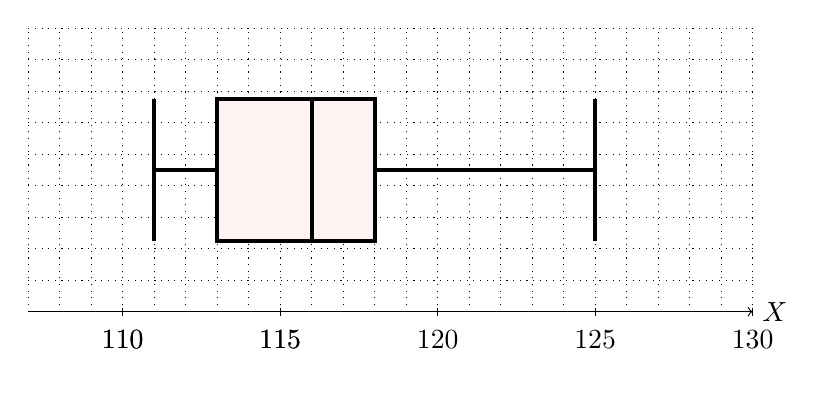
\begin{tikzpicture}[x=0.4cm,y=0.9cm]
         \draw[step=0.4cm,,dotted,color=black] (107,0) grid (130,4);
		\draw[->] (107,0) -- (130,0) node[right] {$X$} ;
		\foreach \X in {110,115,110,115,120,125,130} {
			\draw (\X,0.05cm) -- (\X,-0.05cm) node[below] {$\X\strut$};}
		\draw[ultra thick][fill=red!5] (113,1) rectangle (118,3);
  	\draw[ultra thick] (116,1) -- (116,3);

		\draw[ultra thick] (111,1) -- (111,3);
		\draw[ultra thick] (111,2) -- (113,2);
		\draw[ultra thick] (118,2) -- (125,2);
		%\draw[ultra thick] (4,1) -- (4,3);
		\draw[ultra thick] (125,1) -- (125,3);

			\end{tikzpicture}\\
	\end{center}



Quelle est cette erreur?

  \begin{checkboxes}
\choice La médiane n'est pas au bon endroit.  %  X1
\choice La moyenne échantillonnale n'est pas au bon endroit. % X_2 | X1
\choice Il devrait y avoir deux points: un à 105,5 et un à 125,5.
\choice La moustache de gauche devrait être à  105,5. 
\choice La moustache de droite devrait être à 125,5.
\choice Il n'y a aucune erreur.
\end{checkboxes}

\vspace{1cm}
\newpage
.
\end{questions}


\end{document} 
